\documentclass[a4paper,12pt]{report}

\usepackage[a4paper]{geometry}
\usepackage{amssymb,amsmath,amsthm}
\usepackage{graphicx}
\usepackage{url}
\usepackage{hyperref}
\usepackage{epsfig}
\usepackage[italian]{babel}
\usepackage{setspace}
\usepackage{thesis}
\usepackage{parskip}

\usepackage[utf8]{inputenc}

\newtheorem{lang}{Teorema}[chapter]
\newtheorem{dfa}{Teorema}[chapter]

% FRONTPAGE

\begin{document}
\title{Iperminimizzazione di automi a stati finiti deterministici}
\author{Andrea TINELLI}
\dept{Corso di Laurea in Informatica} 
\anno{2023 - 2024}
\matricola{941800}
\relatore{Prof. Giovanni PIGHIZZINI}

% i think that this is not needed, but i have to verify
% with the professor, to re-enable it: remove the comment
% from the next line and from the thesis.sty file
% \correlatore{nome COGNOME}

% DEDICATIONS

\beforepreface
\prefacesection{}
{\hfill \Large {\sl dedicato a \dots}}



% 
%			PREFAZIONE
%
\prefacesection{Prefazione}
hkjafgyruet.
%
%
%			ORGANIZZAZIONE
\section*{Organizzazione della tesi}
\label{organizzazione}
La tesi \`e organizzata come segue:
\begin{itemize}
\item nel Capitolo 1 ....
\end{itemize}
%
%			RINGRAZIAMENTI
%
\prefacesection{Ringraziamenti}
asdjhgftry.
\afterpreface
% 
% 
%			CAPITOLO 1: dshjkfg
\chapter{Nozioni preliminari}
\label{cap1}

Lo teoria degli automi è uno dei principali e più antichi campi dell'informatica teorica, in questo capitolo, vengono presentati i concetti fondamentali di questo ambito, per una visione più ampia il lettore è rimandato a \cite{HMU06}.

\section{Alfabeti, parole e linguaggi}

Un alfabeto, generalmente indicato con la lettera $\Sigma$, è un insieme finito di simboli, entità astratte non definite formalmente cui esempio possono essere lettere e numeri.

Una parola è una sequenza finita di simboli giustapposti, in particolare, una parola su un alfabeto $\Sigma$ è una sequenza finita di simboli appartenenti a $\Sigma$.

La lunghezza di una parola $w$, indicata con $|w|$, è il numero di simboli che la compongono.
Caso particolare è la parola vuota, a cui per convenzione si fa riferimento con la lettera $\epsilon$, composta da zero simboli ($|\epsilon| = 0$).

Un possibile esempio di alfabeto è $\Sigma = \{0, 1\}$, mentre una possibile parola su $\Sigma$ è $w = 01$, dove $|w| = 2$.

Si è in grado a questo punto di introdurre il concetto di linguaggio.

\begin{lang}\label{th:lang}
  Un linguaggio $L$ su un alfabeto $\Sigma$ è un insieme di parole su $\Sigma$, ovvero, un insieme di parole formate dalla giustappozione di simboli appartenenti a $\Sigma$.
\end{lang}

Due esempi particolari possono essere il linguaggio vuoto $L_\emptyset = \emptyset$ ed il linguaggio composto solo dalla
parola vuota $L_\epsilon = \{\epsilon\}$, puntualizzando il fatto che $L_\emptyset \neq L_\epsilon$,
infatti $|L_\emptyset| = 0$ mentre $|L_\epsilon| = 1$.

Convenzionalmente, fissato un alfabeto $\Sigma$, viene indicato con $\Sigma^*$ il linguaggio composto da tutte
le parole su $\Sigma$, compresa la parola vuota.

Sia $\Sigma = \{a, b\}$, allora $\Sigma^* = \{\epsilon, a, b, aa, ab, ba, bb, aaa, \dots\}$.

\section{Automi}

In generale, un automa è un modello matematico di una macchina che esegue delle operazioni predefinite.

Una delle principali tipologie di automi è quella degli automi a stati finiti (FSA), questi, sono sistemi
con un numero finito di input e output, che possono trovarsi in un numero finito di configurazioni interne chiamate stati.

\begin{dfa}
  \label{th:dfa}
  Un automa a stati finiti deterministico è una quintupla \\
  $A = (Q, \Sigma, \delta, q_I, F)$ dove $Q$ denota un insieme finito di stati, $\Sigma$ un alfabeto, \\
  $\delta: Q \times \Sigma \rightarrow Q$ la funzione di transizione, $q_I \in Q$ lo stato iniziale e $F \subseteq Q$ l'insieme degli stati finali.
\end{dfa}

In Figura \ref{fig:dfa} è mostrato un esmpio di DFA

\begin{figure}[!htb]
  \centering
  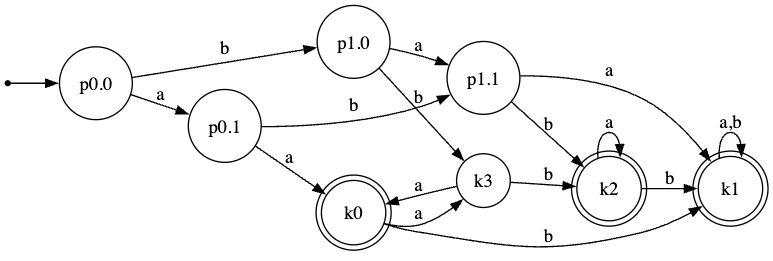
\includegraphics[width=0.7\linewidth]{dfa.png}
  \caption{\label{fig:dfa}This frog was uploaded via the file-tree menu.}
\end{figure}

\section{Minimizzazione}

\chapter{Iperminimizzazione}
\label{cap2}

\section{Decomposizione in preambolo e kernel}
\section{Classi di quasi equivalenza}
\section{Tecniche}
\subsection{Strategia generale}
\subsection{Algoritmo di Badr-Geffert-Shipman}
\subsection{Algoritmo di Badr}
\subsection{Algoritmo di Holzer-Maletti}


\newpage

\cite{BGS09}\cite{Badr}
\cite{HM10}
\cite{DFI08}

\chapter{Implementazione}
\chapter{Risultati sperimentali}

Nel teorema~\ref{th:dfa} abbiamo visto...

% BIBLIOGRAPHY

\bibliographystyle{alpha}
\bibliography{bibliography}

\end{document}


